\chapter{Testing script}
Testing script is one of the core of testing framework.
A testing script can be called a test case.
This chapter describes the components that make up a testing script. At the end of chapter, there are some examples of testing scripts I use for experiments in Chapter \ref{ch:experiments}.

\section{Testing script components}
A testing script consists of one or more script actions. Each script action has following elements:
    \begin{itemize}
		\item[--] \textbf{Source object}: element on the screen to be applied action on
		\item[--] \textbf{Action}: what to do with source object
		\item[--] \textbf{Execution time}: how long it takes to complete the action
		\item[--] \textbf{Expected object} (optional, depended on each action): after finishing action, what expected to be display on the screen
	\end{itemize}

\subsection{Actions}
There are 4 basic actions for robot to apply on mobile phone screen:
    \begin{itemize}
		\item[--] \textbf{Click}: perform a quick single tap on screen
		\item[--] \textbf{Hold}: tap and keep pointer on the screen for a short time then release
		\item[--] \textbf{Drag}: tap on the screen, move pointer to a certain location then release
		\item[--] \textbf{Flick}: tap on the screen and quickly move pointer apart and release
	\end{itemize}

\subsection{States of system}
    \begin{figure}
		\centering
		\includegraphics[scale=0.75]{Chapters/Fig/system_state.png}
		\caption{System state diagram}
		\label{fig:system_state}
	\end{figure}


\subsection{System sequence diagram}
    \begin{figure}
		\centering
		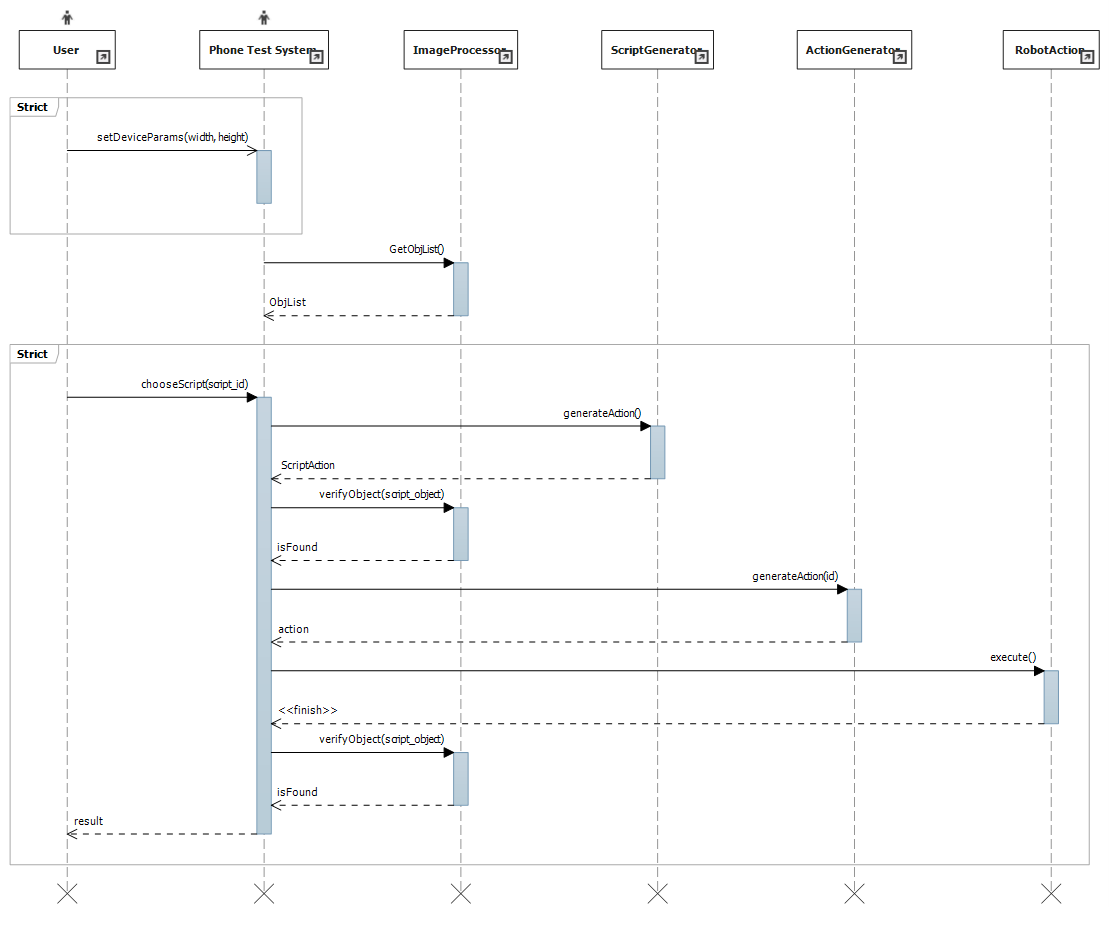
\includegraphics[scale=0.75]{Chapters/Fig/sequence_diagram.png}
		\caption{System sequence diagram}
		\label{fig:sequence_diagram}
	\end{figure}

\subsection{Implementation}
    \begin{figure}
		\centering
		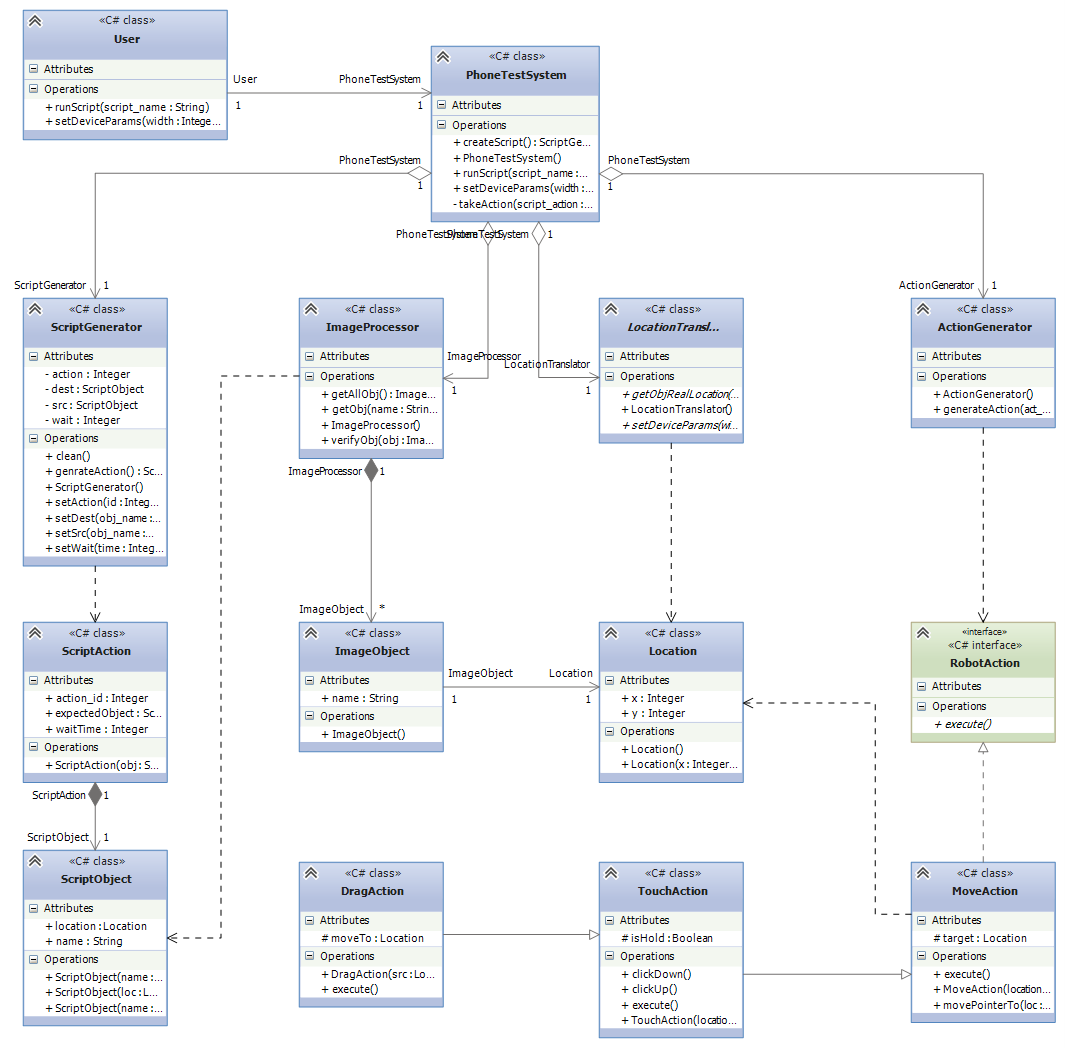
\includegraphics[scale=0.75]{Chapters/Fig/class_diagram.png}
		\caption{System class diagram}
		\label{fig:class_diagram}
	\end{figure}

\section{Testing script example}
\subsection{Simple click test}

\subsection{Set alarm test}